\section{Problem Formulation}
\label{sec:problem}

This section formalizes the task that the rest of the report builds upon: a
team of drones must locate and reach a hidden target on a partially observable
grid, under limited communication, a fixed time budget, and the possibility
that any drone permanently breaks at any moment. We first describe the
scenario informally (Section~\ref{subsec:prob-scenario}), then cast it as a
partially observable Markov game with sequential execution
(Section~\ref{subsec:prob-model}), and detail its three defining ingredients:
the observation model (Section~\ref{subsec:prob-obs}), the communication
model (Section~\ref{subsec:prob-comm}), and the fault model
(Section~\ref{subsec:prob-fault}). Section~\ref{subsec:prob-objective} states
the objective and the reward function that operationalizes it.
Table~\ref{tab:notation} collects the notation used throughout the report.

\begin{table}[t]
\centering
\small
\begin{tabular}{llp{8.6cm}}
\toprule
\textbf{Symbol} & \textbf{Default} & \textbf{Meaning} \\
\midrule
$\mathcal{G}$ & $\{0,\dots,31\}^2$ & set of grid cells (fixed $\gridsize\times\gridsize$ map) \\
$\mathcal{O} \subset \mathcal{G}$, $\rho$ & $\rho \in [0.10, 0.30]$ & obstacle cells and obstacle density \\
$\mathcal{F} = \mathcal{G}\setminus\mathcal{O}$ & --- & free (traversable) cells \\
$g \in \mathcal{F}$ & --- & hidden target cell \\
$\nagents$, $i$ & $\nagents \in \{1,\dots,4\}$ & team size and drone index $i \in \{1,\dots,\nagents\}$ \\
$p_i^t \in \mathcal{F}$ & --- & position of drone $i$ at turn $t$ \\
$\mathcal{A}$ & $\{\mathrm{up},\mathrm{down},\mathrm{left},\mathrm{right}\}$ & action set (4 unit moves) \\
$\rvis$ & $\rvis \in \{1,\dots,6\}$ & vision radius (Chebyshev) \\
$V_i^t \subseteq \mathcal{G}$ & --- & vision set of drone $i$ at turn $t$ \\
$\rcomm$, $d_1$ & $\rcomm \in \{2,\dots,12\}$ & communication range and Manhattan distance \\
$\pfault$ & $\pfault \in [0, 0.003]$ & per-turn fault probability of a live drone \\
$\beta_i^t \in \{0,1\}$ & --- & alive flag of drone $i$ ($0$ = broken, permanent) \\
$K_i^t$ & --- & knowledge state (accumulated maps) of drone $i$ \\
$\mathcal{C}_i^t$, $\hat{n}_i^t$ & --- & crashed teammates \emph{known} to $i$; believed alive count \\
$T_{\max}$ & $200 \cdot \nagents$ & episode budget in agent-turns \\
$\gamma$ & $0.97$ & discount factor \\
\bottomrule
\end{tabular}
\caption{Notation used throughout the report. ``Default'' reports the value
or randomization range used in the final training configuration
(Section~\ref{sec:training}); parameters with a range are resampled at every
episode.}
\label{tab:notation}
\end{table}

\subsection{Scenario}
\label{subsec:prob-scenario}

The environment is an episodic grid world. At the beginning of every episode
a fresh $\gridsize\times\gridsize$ occupancy grid is generated: each cell is
independently declared an obstacle with probability $\rho$, and a single
target cell $g$ is placed uniformly at random among the free cells that are
reachable (under 4-connectivity) from the reference corner
$(0,0)$.\footnote{Reachability is verified with a breadth-first search at
generation time; layouts whose reachable region is empty are rejected and
resampled. The guarantee is stated with respect to the reference corner from
which the search is run.} A team of $\nagents$ drones spawns \emph{co-located}
on one randomly chosen corner of the map. The target position is unknown to
the drones; obstacles are likewise unknown until observed.

Each drone occupies one cell and, on its turn, moves to one of the four
axis-adjacent cells. Drones perceive only a local neighbourhood of their
position (Section~\ref{subsec:prob-obs}), accumulate what they have seen into
a private map, and can merge maps with teammates that are close enough
(Section~\ref{subsec:prob-comm}). The episode succeeds when any drone
\emph{physically reaches} the target cell --- merely spotting the target does
not end the episode, it only reveals its location to the observer (and, via
communication, to nearby teammates). The team operates under a hard budget of
$T_{\max}$ agent-turns; if the budget expires before the target is reached,
the episode fails.

Two features make the problem distinctly harder than classical cooperative
exploration. First, all drones start from the \emph{same} cell, so any
efficient division of the search space must be produced by the drones
themselves --- nothing in the environment assigns regions or roles. Second,
at any turn a live drone may irreversibly break with probability $\pfault$
(Section~\ref{subsec:prob-fault}); the survivors must absorb the loss and
re-cover the region the wreck leaves unsearched, without any central entity
telling them that a teammate is gone.

\subsection{Formal model}
\label{subsec:prob-model}

We model the task as a partially observable Markov game
\citep{littman1994markov,oliehoek2016concise} with identical-interest
(cooperative) structure and \emph{sequential execution},
\[
\mathcal{M} \;=\; \bigl\langle \mathcal{I},\; \mathcal{S},\;
\{\mathcal{A}_i\}_{i \in \mathcal{I}},\; T,\;
\{\mathcal{O}_i\}_{i \in \mathcal{I}},\;
\{r_i\}_{i \in \mathcal{I}},\; \gamma \bigr\rangle ,
\]
where $\mathcal{I} = \{1,\dots,\nagents\}$ is the set of drones and
$\mathcal{A}_i = \mathcal{A}$ for all $i$.

\paragraph{State.}
A global state
$s^t = \bigl(\mathcal{O},\, g,\, (p_i^t)_i,\, (\beta_i^t)_i,\,
(K_i^t)_i,\, t\bigr)$
collects the (episode-fixed) obstacle layout and target position, the drone
positions and alive flags, each drone's knowledge state, and the turn
counter. Including the knowledge states $K_i^t$ in $s^t$ is deliberate: the
per-drone observation is a deterministic rendering of $K_i^t$
(Section~\ref{subsec:prob-obs}), so the process is Markovian in $s^t$, and
partial observability arises precisely from the gap between $K_i^t$ and the
full state. Episode-level parameters
$\theta = (\rvis, \rcomm, \nagents, \rho, \pfault)$ are drawn at the start of
every episode and held fixed within it; their per-episode randomization is a
training-time design choice discussed in Section~\ref{sec:training}.

\paragraph{Sequential execution.}
Time advances in \emph{agent-turns}. At turn $t$ the acting drone is
$\iota(t) = \bigl((t-1) \bmod \nagents\bigr) + 1$, so a \emph{round} consists
of $\nagents$ consecutive turns in fixed order. Only the acting drone selects
an action; every other drone's position is unchanged. Crucially, a turn is
consumed \emph{even when the acting drone is broken}
(Section~\ref{subsec:prob-fault}): the clock never skips, so losing drones
never stretches the time budget. Sequential execution gives collisions and
map updates an unambiguous semantics (there are no simultaneous-move
conflicts to resolve) and matches the execution model of the learning
architecture, where all drones are driven by a single shared network
(Section~\ref{sec:architecture}).

\paragraph{Transition.}
The transition kernel $T$ composes a stochastic fault event with a
deterministic move. At the start of its turn, a live acting drone $i$ breaks
with probability $\pfault$ (its position freezes, $\beta_i \leftarrow 0$,
permanently). Otherwise it executes its action: the move succeeds if the
destination cell is inside the grid and not an obstacle, and the drone stays
in place if it is not. After moving, the drone's vision, the fault-beacon
detection, and the communication fusion update the knowledge states
(Sections~\ref{subsec:prob-obs}--\ref{subsec:prob-fault}). The only sources
of stochasticity are the episode initialization (layout, target, spawn
corner, $\theta$) and the fault process.

\paragraph{Action masking.}
The acting drone receives a binary mask over $\mathcal{A}$ that disables
moves leaving the grid or entering an obstacle in one of the four adjacent
cells. Because $\rvis \geq 1$, the adjacent cells are always inside the
drone's current vision set, so the mask adds no information beyond what the
drone has already observed --- it merely removes actions whose outcome
(bouncing in place) is already known, shrinking the exploration space. A
safety fallback re-enables all actions in the degenerate case where a drone
is boxed in on all four sides, guaranteeing the policy always has a legal
choice.

\paragraph{Episode end.}
The episode \emph{terminates} (success) as soon as the acting drone's new
position equals $g$. It is \emph{truncated} (failure) when $t$ exceeds
$T_{\max} = 200\cdot\nagents$, or early when all drones are broken, since no
state change is possible anymore. The distinction between termination and
truncation is not cosmetic: it changes the bootstrapping semantics of the
learning update, and Section~\ref{subsec:train-correctness} argues that
treating faults and time-outs as truncations is necessary for unbiased value
estimation.

\subsection{Observation model}
\label{subsec:prob-obs}

Each drone senses a square window centred on itself: at turn $t$, drone $i$'s
vision set is the Chebyshev ball
\[
V_i^t \;=\; \bigl\{\, c \in \mathcal{G} \;:\;
\lVert c - p_i^t \rVert_\infty \le \rvis \,\bigr\},
\]
i.e.\ a $(2\rvis{+}1)\times(2\rvis{+}1)$ box clipped to the grid. Sensing is
noiseless but strictly local: nothing outside $V_i^t$ is perceived.

What the policy consumes, however, is not the instantaneous percept but an
\emph{accumulated knowledge state}. Drone $i$ maintains
$K_i^t = (\mathit{Vis}_i, \mathit{Obs}_i, \mathit{Tgt}_i, \tau_i,
\mathit{Brk}_i, \mathcal{C}_i)$, a set of spatial maps over $\mathcal{G}$
updated after every move: for every cell $c \in V_i^t$,
\[
\mathit{Obs}_i(c) \leftarrow 1 \;\; \text{if } c \in \mathcal{O}, \qquad
\mathit{Tgt}_i(c) \leftarrow 1 \;\; \text{if } c = g, \qquad
\mathit{Vis}_i(c) \leftarrow 1 \;\; \text{otherwise}.
\]
All three maps are monotone --- knowledge is never forgotten, so a target
spotted once remains marked even after it leaves the field of view. The
trajectory map $\tau_i(c)$ counts how many times drone $i$ itself has
occupied cell $c$; unlike the other maps it is \emph{private}
(never communicated), acting as a personal revisit memory. The crash-site
map $\mathit{Brk}_i$ and the crashed-teammate set $\mathcal{C}_i$ record
fault knowledge and are described in Section~\ref{subsec:prob-fault}.

The observation $o_i^t \in \mathcal{O}_i$ delivered to the policy is a
deterministic, multi-channel rendering of $K_i^t$ plus the drone's own
position and the positions of \emph{live} teammates currently inside
$V_i^t$; its exact tensor encoding is an architectural matter deferred to
Section~\ref{subsec:arch-obs}. Conceptually, the accumulated maps play the
role of a hand-crafted belief state: they compress the interaction history
into a spatial summary, which is what allows a memoryless (non-recurrent)
policy to act reasonably in a partially observable world.

\subsection{Communication model}
\label{subsec:prob-comm}

Communication is proximity-bound, instantaneous, and content-fixed: what is
exchanged is \emph{world knowledge}, never commands or intentions. After
every turn, consider the communication graph over live drones with an edge
between $i$ and $j$ whenever their Manhattan distance satisfies
$d_1(p_i^t, p_j^t) \le \rcomm$. For every connected component $S$ of this
graph, the members merge their knowledge by an element-wise maximum,
\[
\mathit{Vis}_i \leftarrow \max_{j \in S} \mathit{Vis}_j, \qquad
\mathit{Obs}_i \leftarrow \max_{j \in S} \mathit{Obs}_j, \qquad
\mathit{Tgt}_i \leftarrow \max_{j \in S} \mathit{Tgt}_j, \qquad
\mathit{Brk}_i \leftarrow \max_{j \in S} \mathit{Brk}_j,
\]
together with the union of the crashed-teammate sets
$\mathcal{C}_i \leftarrow \bigcup_{j \in S} \mathcal{C}_j$, for every
$i \in S$. Merging over connected components makes communication
\emph{transitive} within a round: if $A$ is in range of $B$ and $B$ of $C$,
all three end up with identical fused maps even if $A$ and $C$ are far
apart --- intermediate drones act as relays.

Three properties of this mechanism are worth stressing, as they carry the
multi-agent analysis of Section~\ref{sec:mas}. First, fusion is
\emph{anonymous}: the max-merge keeps no record of who contributed which
cell, so shared knowledge detaches from its producer. Second, it is
\emph{persistent}: knowledge received in an encounter survives after the
drones part ways, because it is written into the receiver's own maps. Third,
it is \emph{selective}: the trajectory map $\tau_i$ is deliberately excluded
from fusion, so the revisit-avoidance signal remains individual. Wrecks
neither transmit nor receive --- a broken drone's maps freeze at fault time.

\subsection{Fault model}
\label{subsec:prob-fault}

The defining extension of this project is a random, permanent fault process.
At the start of its own turn, a live drone breaks with probability
$\pfault$, independently across drones and turns. The values used in
training are small per-turn probabilities with large episode-level effect:
at $\pfault = 0.003$ over $200$ rounds, a given drone breaks at some point
of the episode with probability $1 - 0.997^{200} \approx 0.45$.

A broken drone (a \emph{wreck}) is subject to the following semantics:

\begin{itemize}[leftmargin=1.5em]
  \item \textbf{Total incapacitation.} It no longer moves, senses, or
    communicates; its knowledge state freezes at fault time.
  \item \textbf{No time refund.} Its turns still occur and still consume the
    shared budget $T_{\max}$: the team loses capacity but gains no time.
  \item \textbf{Physically inert.} The crash cell is not an obstacle: live
    drones can traverse it, it never blocks a corridor (which preserves the
    reachability guarantee of the target), and the wreck is excluded from
    collision counting and from teammate-position observations.
\end{itemize}

\paragraph{Decentralized fault knowledge.}
No drone is notified of a teammate's fault. Instead, a wreck passively emits
a \emph{distress beacon}: a live drone $i$ discovers crash site $c_j$ of
drone $j$ when it either comes within communication range of it,
$d_1(p_i^t, c_j) \le \rcomm$, or sees it, $c_j \in V_i^t$. Upon detection,
$i$ records the crash in its own maps,
$\mathit{Brk}_i(c_j) \leftarrow 1$ and
$\mathcal{C}_i \leftarrow \mathcal{C}_i \cup \{j\}$, and this knowledge then
spreads through the ordinary map fusion of
Section~\ref{subsec:prob-comm} exactly like any other observation. Each
drone therefore holds a \emph{belief} about the team's size,
\[
\hat{n}_i^t \;=\; \nagents - \lvert \mathcal{C}_i^t \rvert ,
\]
which is sound but possibly stale: since $\mathcal{C}_i^t$ can only contain
drones that actually crashed, $\hat{n}_i^t$ never underestimates the true
alive count, but it may overestimate it for many rounds if the crash
happened far away. There is no global fault oracle anywhere in the system:
every quantity a drone acts upon --- including $\hat{n}_i^t$, which is fed
to the policy (Section~\ref{subsec:arch-context}) --- is derived from that
drone's own observations and from what teammates relayed to it. When the
last drone breaks, the episode is truncated early.

For learning purposes a fault is treated as a \emph{truncation} of the
broken drone's experience stream, not as a terminal state: the fault strikes
independently of the drone's state and action, and
Section~\ref{subsec:train-correctness} shows why conflating the two would
bias the learned values.

\begin{figure}[t]
\centering
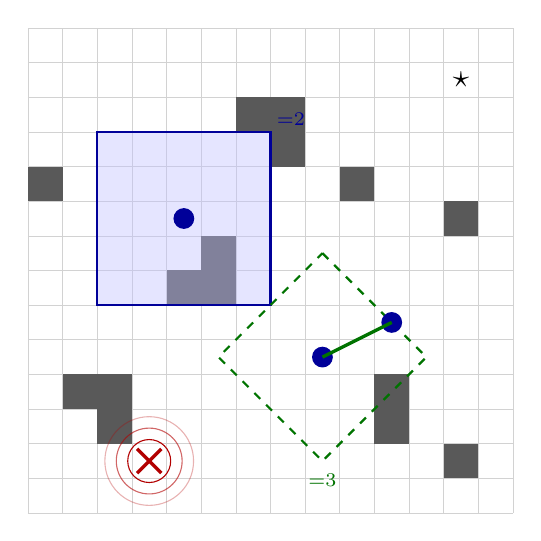
\begin{tikzpicture}[scale=0.44]
  % --- board ---
  \draw[step=1, gray!35, very thin] (0,0) grid (14,14);
  % --- obstacles ---
  \foreach \pos in {(1,3),(2,3),(2,2),(6,11),(7,11),(7,10),(10,2),(10,3),
                    (4,6),(5,6),(5,7),(12,8),(0,9),(9,9),(12,1)}
    \fill[black!65] \pos rectangle +(1,1);
  % --- hidden target ---
  \node at (12.5,12.5) {\large $\star$};
  % --- drone i: vision box (Chebyshev, r_vis = 2) ---
  \fill[blue!25, opacity=0.4] (2,6) rectangle (7,11);
  \draw[blue!60!black, thick] (2,6) rectangle (7,11);
  \fill[blue!60!black] (4.5,8.5) circle (0.30);
  \node[blue!60!black, anchor=south west] at (6.9,10.9) {\scriptsize $\rvis{=}2$};
  % --- drones j,k: comm range (Manhattan, r_comm = 3) ---
  \draw[green!45!black, thick, dashed] (8.5,7.5) -- (11.5,4.5) -- (8.5,1.5) -- (5.5,4.5) -- cycle;
  \fill[blue!60!black] (8.5,4.5) circle (0.30);
  \fill[blue!60!black] (10.5,5.5) circle (0.30);
  \draw[green!45!black, very thick] (8.5,4.5) -- (10.5,5.5);
  \node[green!45!black, anchor=north] at (8.5,1.4) {\scriptsize $\rcomm{=}3$};
  % --- wreck + distress beacon ---
  \draw[red!70!black, very thick] (3.15,1.15) -- (3.85,1.85);
  \draw[red!70!black, very thick] (3.15,1.85) -- (3.85,1.15);
  \draw[red!70!black] (3.5,1.5) circle (0.62);
  \draw[red!70!black, opacity=0.6] (3.5,1.5) circle (0.95);
  \draw[red!70!black, opacity=0.3] (3.5,1.5) circle (1.28);
\end{tikzpicture}
\caption{Schematic of the search scenario (illustrative $14\times14$ crop;
the actual map is $\gridsize\times\gridsize$). Dark cells are obstacles and
$\star$ is the hidden target. The left drone's square outline is its
Chebyshev vision window ($\rvis = 2$), inside which cells are revealed and
accumulated into its private map. The dashed diamond is the Manhattan
communication ball ($\rcomm = 3$) of the lower drone: the teammate inside it
fuses maps with it on every turn (solid link). The red cross is a wreck; its
concentric rings depict the distress beacon, which live drones detect when
they come within $\rcomm$ of the crash site (or see it), with no global
notification of the fault.}
\label{fig:scenario}
\end{figure}

\subsection{Objective and metrics}
\label{subsec:prob-objective}

The team's objective is to minimize the time at which the target is first
reached --- equivalently, to maximize the probability of reaching it within
the budget and, among successful strategies, to reach it as early as
possible. The task is identical-interest: no drone has a private goal, and
it is irrelevant \emph{which} drone reaches the target.

\begin{table}[t]
\centering
\small
\begin{tabular}{llll}
\toprule
\textbf{Term} & \textbf{Symbol} & \textbf{Value} & \textbf{Applied when} \\
\midrule
step penalty & $r_{\mathrm{step}}$ & $-0.3$ & every turn of a live drone (base cost of time) \\
wall penalty & $r_{\mathrm{wall}}$ & $-0.02$ & the move is invalid; the drone stays in place \\
revisit penalty & $r_{\mathrm{rev}} \cdot k$ & $-0.05 \cdot k$ & entering a cell drone $i$ already visited $k$ times \\
collision penalty & $r_{\mathrm{coll}} \cdot m$ & $-0.5 \cdot m$ & entering a cell occupied by $m$ other live drones \\
exploration bonus & $r_{\mathrm{expl}} \cdot c$ & $+0.02 \cdot c$ & $c$ cells newly added to the \emph{team's} discovered set \\
target reward & $R_{\mathrm{tgt}}$ & $+200$ & the drone's new cell is the target (terminates) \\
\bottomrule
\end{tabular}
\caption{Reward terms accumulated within a single turn of the acting drone
(values from the final configuration). Wrecks receive no reward: their turns
are no-ops.}
\label{tab:reward}
\end{table}

This objective is operationalized by the shaped per-turn reward of
Table~\ref{tab:reward}. On its turn, a live drone $i$ collects
\[
r_i^t \;=\; r_{\mathrm{step}}
\;+\; \mathbb{1}[\text{invalid move}]\, r_{\mathrm{wall}}
\;+\; \mathbb{1}[\text{valid move}] \bigl( k \, r_{\mathrm{rev}} + m \, r_{\mathrm{coll}} \bigr)
\;+\; c \, r_{\mathrm{expl}}
\;+\; \mathbb{1}[p_i^{t} = g]\, R_{\mathrm{tgt}} ,
\]
and the learning objective is the usual expected discounted return with
discount $\gamma$. Each term implements one facet of the task:

\begin{itemize}[leftmargin=1.5em]
  \item \emph{Time pressure.} The constant step penalty makes every turn
    costly, so faster target acquisition strictly dominates.
  \item \emph{Efficient coverage.} The exploration bonus counts cells that
    are new \emph{to the team} (the union of all discovered sets), not to
    the individual: re-discovering a region a teammate already swept earns
    nothing, which rewards complementary --- rather than duplicated ---
    search.
  \item \emph{Revisit avoidance.} The revisit penalty is linear in the
    drone's own prior visit count $k$ of the destination cell, so the
    cumulative cost of oscillating on the same spot grows quadratically with
    the number of passes; pacing back and forth is increasingly expensive.
  \item \emph{Dispersion.} The collision penalty charges co-location with
    live teammates. Since all drones spawn on the same corner, this is the
    only signal pushing the team to split; no region assignment or
    coordination protocol is provided (a point developed in
    Section~\ref{subsec:mas-coordination}).
  \item \emph{Team credit.} With the cooperative credit-assignment variant
    used in the final configuration (\texttt{shared\_target\_reward}), the
    terminal bonus $R_{\mathrm{tgt}}$ is granted to the whole surviving
    team rather than only to the finder, aligning individual returns with
    the identical-interest objective; drones that broke before the find are
    excluded. The learning-side implications of this choice are discussed in
    Section~\ref{subsec:train-correctness}.
\end{itemize}

At evaluation time (Section~\ref{sec:experiments}) the reward is set aside
and performance is reported through task-level metrics: \emph{success rate}
(fraction of episodes in which the target is reached within $T_{\max}$),
\emph{time-to-find} (turns elapsed at termination, over successful
episodes), \emph{coverage} (fraction of free cells discovered by the team),
and \emph{redundancy} (overlap between the regions swept by different
drones). The last two also serve as quantitative signatures of the emergent
division of labour analysed in Section~\ref{subsec:mas-emergence}.

% TODO (figures pass): consider adding a GUI screenshot next to the TikZ
% schematic once final visuals are ready.
